Do wyznaczenia odometrii pojazdu wymagane są enkodery, dlatego w~celu
stworzenia projektu, który będzie łatwy do integracji z~rzeczywistym pojazdem,
zasymulowano pomiary z enkodera.
Pomiary z enkodera pobierane są w ten sposób, że porównywane są w~czasie
kolejne dwa odczyty z kąta obrotu osi koła.
Na tej podstawie otrzymujemy prędkość kątową danego koła.

Część symulująca odczyt z autoenkodera została zaimplementowana jako osobny
węzeł w architekturze platformy ROS.
Węzeł autoenkodera komunikuje się z~węzłem który jest odpowiedzialny za
wyznaczanie poszczególnych parametrów,
określających odometrię pojazdu.
Parametry, czyli model kinematyczny robota, został opisany w kolejnym
podrozdziale.

\section{Model kinematyczny robota}
\begin{figure}
  \centering
  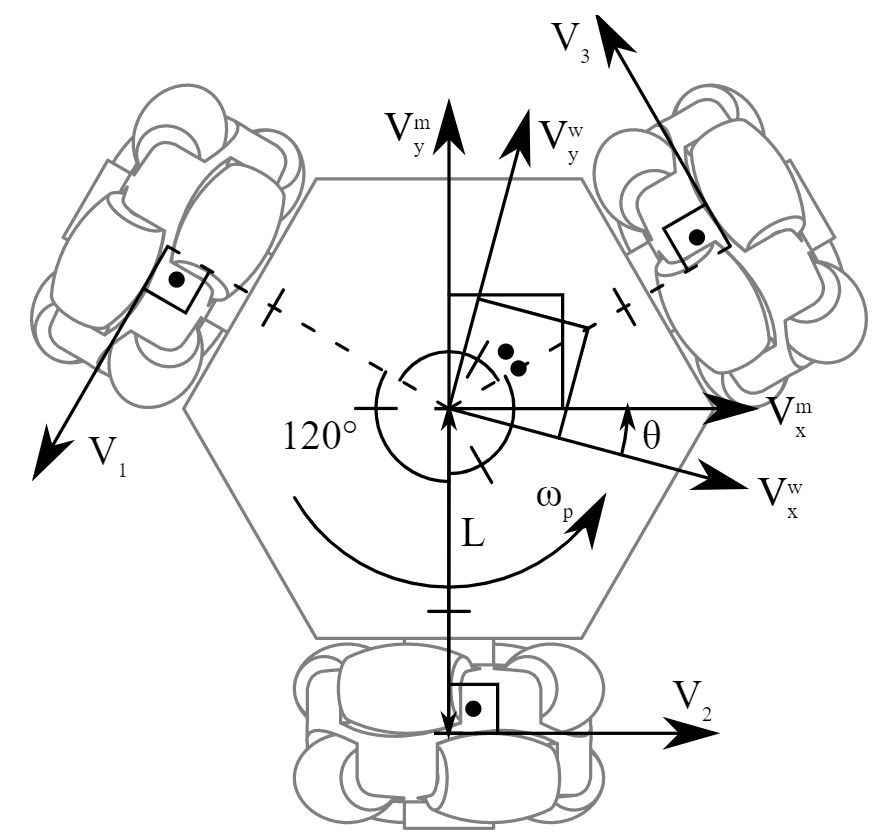
\includegraphics[width=100mm]{graphics/omnischeme.png}
  \caption{Schemat ukazujący poszczególne wektory prędkości}
  \label{fig:forklift}
\end{figure}

Równania kinematyczne odnoszące się do punktu odniesienia robota:
\begin{gather*}
 V_x^m = \frac{2 \cdot V_2 - V_1 - V_3}{3} \\
 V_y^m = \frac{\sqrt{3} \cdot V_3 - \sqrt{3} \cdot V_1}{3} \\
 \omega_p = \frac{V_1 + V_2 + V_3}{3 \cdot L}
\end{gather*}

Równania kinematyczne odnoszące się do punktu odniesienia świata:
\begin{gather*}
 V_x^w = \cos{\theta} \cdot V_x^m - \sin{\theta} \cdot V_y^m\\
 V_y^w = \sin{\theta} \cdot V_x^m + \cos{\theta} \cdot V_y^m\\
\end{gather*}

Kinematyka odwrotna w układzie odniesienia robota:
\begin{gather*}
 V_x^m = \cos{\theta} \cdot V_x^m + \sin{\theta} \cdot V_y^m\\
 V_y^m = -\sin{\theta} \cdot V_x^m + \cos{\theta} \cdot V_y^m\\
\end{gather*}

Kinematyka odwrotna w układzie odniesienia świata:
\begin{gather*}
 V_1 = - \frac{V_x^m}{2} - \frac{\sqrt{3} \cdot V_y^m}{2} + L \cdot \omega_p \\
 V_2 = V_x^m + L \cdot \omega_p \\
 V_3 = - \frac{V_x^m}{2} + \frac{\sqrt{3} \cdot V_y^m}{2} + L \cdot \omega_p
\end{gather*}

Za pomocą powyższych wzorów modelu kinematycznego pojazdu, zrealizowano
odometrię oraz sterowaniem robotem.
